\documentclass[tikz,border=6pt]{standalone}
\usepackage{fontspec}
\setmainfont{Noto Sans}
\usepackage{amsmath,amssymb}
\usepackage{tikz}
\usetikzlibrary{arrows.meta,positioning,calc}
\definecolor{cudaG}{RGB}{118,185,0}
\definecolor{sadRed}{RGB}{200,60,50}
\definecolor{gsBlue}{RGB}{40,110,190}
\definecolor{pyYel}{RGB}{240,170,30}
\definecolor{bgGray}{RGB}{242,242,242}
\begin{document}
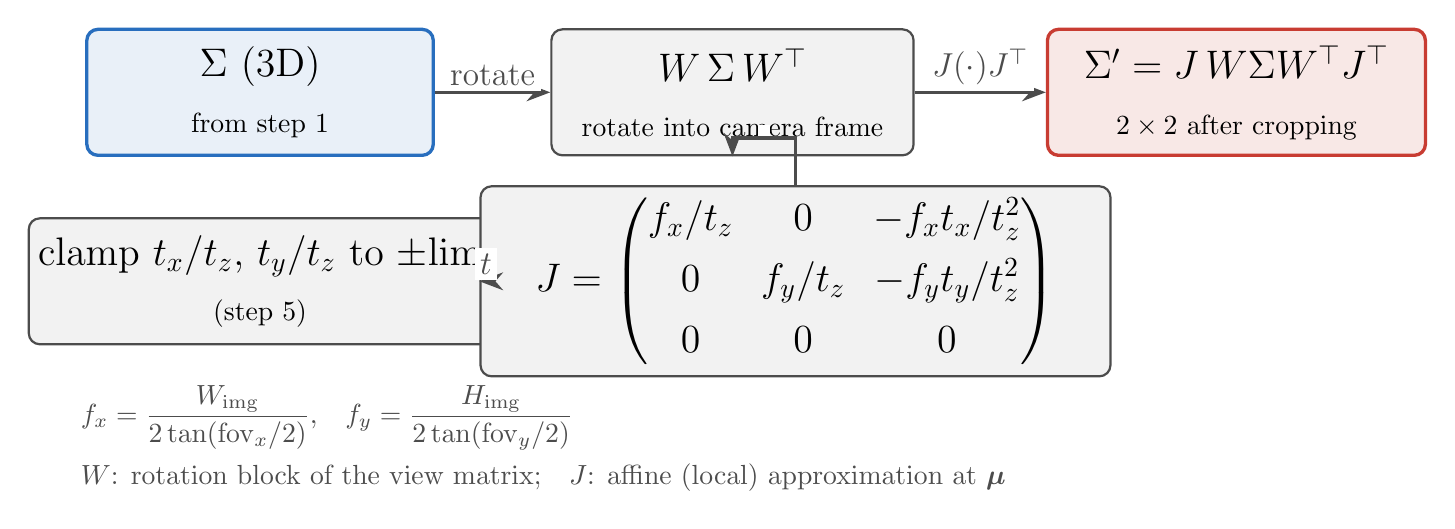
\begin{tikzpicture}[
  inp/.style={draw=gsBlue, very thick, rounded corners, fill=gsBlue!10, minimum width=4.4cm, minimum height=1.6cm, align=center, font=\Large},
  stp/.style={draw=black!70, thick, rounded corners, fill=bgGray, minimum width=4.6cm, minimum height=1.6cm, align=center, font=\Large},
  outb/.style={draw=sadRed, very thick, rounded corners, fill=sadRed!12, minimum width=4.8cm, minimum height=1.6cm, align=center, font=\Large},
  arr/.style={-{Stealth[length=3mm]}, very thick, black!70},
  lab/.style={font=\large, text=black!70, fill=white, inner sep=2pt}
]
  % top row: data flow
  \node[inp] (S3) at (0,4) {$\Sigma$ (3D)\\[2pt]{\normalsize from step 1}};
  \node[stp] (WSW) at (6,4) {$W\,\Sigma\,W^{\top}$\\[2pt]{\normalsize rotate into camera frame}};
  \node[outb] (S2) at (12.4,4) {$\Sigma'=J\,W\Sigma W^{\top}J^{\top}$\\[2pt]{\normalsize $2\times2$ after cropping}};

  \draw[arr] (S3) -- node[lab,above] {rotate} (WSW);
  \draw[arr] (WSW) -- node[lab,above] {$J(\cdot)J^{\top}$} (S2);

  % middle: Jacobian
  \node[stp] (cl) at (0,1.6) {clamp $t_x/t_z$, $t_y/t_z$ to $\pm\mathrm{lim}$\\[2pt]{\normalsize (step 5)}};
  \node[stp, minimum width=8cm] (J) at (6.8,1.6) {$J=\begin{pmatrix} f_x/t_z & 0 & -f_x t_x/t_z^{2}\\[4pt] 0 & f_y/t_z & -f_y t_y/t_z^{2}\\[4pt] 0&0&0\end{pmatrix}$};

  \draw[arr] (cl) -- node[lab,above] {$t$} (J);
  \draw[arr] (J.north) -- ($(J.north)+(0,0.6)$) -| node[lab, pos=0.25, above] {} (WSW.south);

  % bottom: focal lengths and final crop
  \node[font=\normalsize, text=black!70, align=left, anchor=west] at (-2.4,-0.4)
    {$f_x=\dfrac{W_{\mathrm{img}}}{2\tan(\mathrm{fov}_x/2)}$,\quad $f_y=\dfrac{H_{\mathrm{img}}}{2\tan(\mathrm{fov}_y/2)}$\\[4pt]
     $W$: rotation block of the view matrix;\quad $J$: affine (local) approximation at $\boldsymbol{\mu}$};
\end{tikzpicture}
\end{document}
